% lucid_printing.Rnw
% Time-stamp: <15 Dec 2014 17:59:43 c:/x/rpack/lucid/vignettes/lucid_printing.Rnw>

% \VignetteEngine{knitr::knitr}
% \VignetteIndexEntry{Lucid printing}

\documentclass[12pt]{article}\usepackage[]{graphicx}\usepackage[]{color}
%% maxwidth is the original width if it is less than linewidth
%% otherwise use linewidth (to make sure the graphics do not exceed the margin)
\makeatletter
\def\maxwidth{ %
  \ifdim\Gin@nat@width>\linewidth
    \linewidth
  \else
    \Gin@nat@width
  \fi
}
\makeatother

\definecolor{fgcolor}{rgb}{0.345, 0.345, 0.345}
\newcommand{\hlnum}[1]{\textcolor[rgb]{0.686,0.059,0.569}{#1}}%
\newcommand{\hlstr}[1]{\textcolor[rgb]{0.192,0.494,0.8}{#1}}%
\newcommand{\hlcom}[1]{\textcolor[rgb]{0.678,0.584,0.686}{\textit{#1}}}%
\newcommand{\hlopt}[1]{\textcolor[rgb]{0,0,0}{#1}}%
\newcommand{\hlstd}[1]{\textcolor[rgb]{0.345,0.345,0.345}{#1}}%
\newcommand{\hlkwa}[1]{\textcolor[rgb]{0.161,0.373,0.58}{\textbf{#1}}}%
\newcommand{\hlkwb}[1]{\textcolor[rgb]{0.69,0.353,0.396}{#1}}%
\newcommand{\hlkwc}[1]{\textcolor[rgb]{0.333,0.667,0.333}{#1}}%
\newcommand{\hlkwd}[1]{\textcolor[rgb]{0.737,0.353,0.396}{\textbf{#1}}}%

\usepackage{framed}
\makeatletter
\newenvironment{kframe}{%
 \def\at@end@of@kframe{}%
 \ifinner\ifhmode%
  \def\at@end@of@kframe{\end{minipage}}%
  \begin{minipage}{\columnwidth}%
 \fi\fi%
 \def\FrameCommand##1{\hskip\@totalleftmargin \hskip-\fboxsep
 \colorbox{shadecolor}{##1}\hskip-\fboxsep
     % There is no \\@totalrightmargin, so:
     \hskip-\linewidth \hskip-\@totalleftmargin \hskip\columnwidth}%
 \MakeFramed {\advance\hsize-\width
   \@totalleftmargin\z@ \linewidth\hsize
   \@setminipage}}%
 {\par\unskip\endMakeFramed%
 \at@end@of@kframe}
\makeatother

\definecolor{shadecolor}{rgb}{.97, .97, .97}
\definecolor{messagecolor}{rgb}{0, 0, 0}
\definecolor{warningcolor}{rgb}{1, 0, 1}
\definecolor{errorcolor}{rgb}{1, 0, 0}
\newenvironment{knitrout}{}{} % an empty environment to be redefined in TeX

\usepackage{alltt}
% Note, 11 pt fails with a missing font unless we have \usepackage{ae}

\usepackage{color}
\definecolor{navy}{rgb}{0,0,0.5}
\definecolor{maroon}{rgb}{0.6,0.0,0.0}
\definecolor{lightgray}{rgb}{0.7,0.7,0.7}

\usepackage[colorlinks,citecolor=navy,linkcolor=navy,urlcolor=navy]{hyperref}

%\usepackage{url}     % Don't break long URLs
\raggedright         % Don't right-justify
\usepackage{parskip} % Extra vertical space between paragraphs

\usepackage{enumitem}
\setlist{nolistsep}  % Reduce spacing between list items

\usepackage[left=.5in,top=.5in,right=.5in,bottom=1in]{geometry}

\newcommand{\code}[1]{\texttt{\textcolor{maroon}{#1}}}

% Header & footer
\usepackage{titling} % copy \title{} into \thetitle
\usepackage{fancyhdr}
\pagestyle{fancy}
\renewcommand{\headrule}{}  % no line between header and body
\renewcommand{\footrule}{}  % no line between body and footer
\fancyhf{} % clear header and footer fields
\fancyfoot[L]{\small \color{lightgray} \thetitle}
\fancyfoot[R]{\small \thepage}

\usepackage[round]{natbib}
% plainnat to include url's in bibliography.  Authors first name is first
% apalike does NOT handle urls
\bibliographystyle{plainnat}

\renewcommand{\familydefault}{\sfdefault} % Use arial everywhere
% Load this AFTER arial and it will redefine tt family to use inconsolata.
\IfFileExists{zi4.sty}{\usepackage[noupquote]{zi4}}{\usepackage{inconsolata}}

% ----------------------------------------------------------------------------
\IfFileExists{upquote.sty}{\usepackage{upquote}}{}
\begin{document}

\title{Lucid printing}
\author{Kevin Wright}
\maketitle
\thispagestyle{fancy}

% Setup stuff.

% ----------------------------------------------------------------------------

\section{Abstract}

The \code{lucid} package provides a method for pretty-printing vectors
of floating point numbers, with special application to
printing of variance components from mixed models.


% ----------------------------------------------------------------------------
\section{Intro}

Numerical output from R is often in scientific notation, which can make it
difficult to quickly glance at numbers and understand the relative sizes
of the numbers.  This not a new phenomenon.  Before R had been created,
\cite[351-352]{finney1988data} had this to say about numerical output:
\begin{quote}
Certainly, in initiating analyses by standard software or in writing one's
own software, the aim should be to have output that is easy to read and easily
intelligible to others. ... Especially undesirable is the so-called
'scientific notation' for numbers in which every number is shown as a value
between 0.0 and 1.0 with a power of 10 by which it must be multiplied. For
example:
\begin{verbatim}
0.1234E00 is 0.1234
0.1234E02 is 12.34
0.1234E-1 is 0.01234
\end{verbatim}
This is an abomination which obscures the comparison of related quantities;
tables of means or of analyses of variance become very difficult to read. It
is acceptable as a default when a value is unexpectedly very much larger or
smaller than its companions, but its appearance as standard output denotes
either lazy programming or failure to use good software properly. Like
avoidance of 'E', neat arrangement of output values in columns, with decimal
points on a vertical line, requires extra effort by a programmer but should be
almost mandatory for any software that is to be used often.
\end{quote}

One recommendation for improving the display of tables of numbers
is to round numbers a lot \citep{wainer1997improving}.  Humans cannot
understand more than two digits very easily.  It is rare that more
than two digits of accuracy can be justified, and even if we could justify
more than two digits, we seldom care about more than two digits.
In R, using the \code{round} and \code{signif} functions can help improve
numerical output, but can still print results in scientific notation
and leave much to be desired.
The \code{lucid} package provides functions to improve the presentation of
floating point numbers in a way that makes interpretation of the numbers
{\bf immediately} apparent.

Consider the following vector of coefficients from a fitted model:
\begin{knitrout}
\definecolor{shadecolor}{rgb}{0.969, 0.969, 0.969}\color{fgcolor}\begin{kframe}
\begin{verbatim}
##                    effect
## A           -1.350000e+01
## B            4.500000e+00
## C            2.450000e+01
## C1           6.927792e-14
## C2          -1.750000e+00
## D            1.650000e+01
## (Intercept)  1.135000e+02
\end{verbatim}
\end{kframe}
\end{knitrout}
Which coeficient is basically zero?  How large is the intercept?

Both questions can be answered using the output shown above, but it
takes too much effort to answer the questions.  Now examine the same
vector of coefficients with prettier formatting:
\begin{knitrout}
\definecolor{shadecolor}{rgb}{0.969, 0.969, 0.969}\color{fgcolor}\begin{kframe}
\begin{alltt}
\hlkwd{require}\hlstd{(}\hlstr{"lucid"}\hlstd{)}
\hlkwd{options}\hlstd{(}\hlkwc{digits}\hlstd{=}\hlnum{7}\hlstd{)} \hlcom{# knitr defaults to 4, R console uses 7}
\hlkwd{lucid}\hlstd{(df1)}
\end{alltt}
\begin{verbatim}
##             effect
## A           -13.5 
## B             4.5 
## C            24.5 
## C1            0   
## C2           -1.75
## D            16.5 
## (Intercept) 114
\end{verbatim}
\end{kframe}
\end{knitrout}
Which coeficient is basically zero?  How large is the intercept?

Printing the numbers with the \code{lucid} function has made the
questions much easier to answer.


The sequence of steps used by \code{lucid} to format and
print the output is.
\begin{enumerate}
\item{Zap to zero}
\item{Round using significant digits}
\item{Drop trailing zeros}
\item{Align numbers at the decimal point}
\end{enumerate}

The \code{lucid} package contains a generic function \code{lucid} with
specific methods for numeric vectors, matrices, lists and data frames.
The methods for matrices and data frames apply formatting to each
numeric column and leave other columns unchanged.


% Look at the raw/lucid table of variance components below.
% Which are the smallest/largest/significant variance components?
% <<echo=FALSE>>=
% df2 <- data.frame(effect=c('hyb','region','region:loc','hyb:region','yr','hyb:yr','region:yr','residual'),
%                   component=c(10.9,277,493,1.30E-04,126,22.3,481,268),
%                   std.error=c(4.40,166,26.1,1.58E-06,119,4.50,108,3.25),
%                   z.ratio=c(2.471,1.669,18.899,82.242,1.060,4.951,4.442,82.242),
%                   constraint=c('pos','pos','pos','bnd','pos','pos','pos','pos'))
% print(df2)
% @
% <<echo=TRUE>>=
% lucid(df2)
% @

%Note the similarity in overall shape of the positions of the leftmost
%significant digit in the 'component' column of the lucid output and
%the dotplot of the components on a log10 scale.  See \cite{gelman2011tables}.
%<<fig.height=4>>=
%df2$effect <- factor(df2$effect, levels=rev(df2$effect))
%require(lattice)
%dotplot(effect~ log10(component), data=df2,
%        cex=1, xlim=c(3,-4), xlab="variance component (log10 scale)",
%        scales=list(x=list(lab=rev(c('1000','100','10','1','.1','.01','.001'
%,'.0001')))))
%@


% ----------------------------------------------------------------------------

\section{Example: Antibiotic effectiveness}

\cite{wainer2009pictures} present data published by Will Burtin in 1951
on the effectiveness of antibiotics against 16 types of bacteria.
The data is included in the \code{lucid} package as a dataframe
called \code{antibiotic}.  The default view of this data is:
\begin{knitrout}
\definecolor{shadecolor}{rgb}{0.969, 0.969, 0.969}\color{fgcolor}\begin{kframe}
\begin{alltt}
\hlkwd{print}\hlstd{(antibiotic)}
\end{alltt}
\begin{verbatim}
##                           bacteria penicillin streptomycin neomycin gramstain
## 1             Aerobacter aerogenes    870.000         1.00    1.600       neg
## 2                 Brucella abortus      1.000         2.00    0.020       neg
## 3                Brucella antracis      0.001         0.01    0.007       pos
## 4           Diplococcus pneumoniae      0.005        11.00   10.000       pos
## 5                 Escherichia coli    100.000         0.40    0.100       neg
## 6            Klebsiella pneumoniae    850.000         1.20    1.000       neg
## 7       Mycobacterium tuberculosis    800.000         5.00    2.000       neg
## 8                 Proteus vulgaris      3.000         0.10    0.100       neg
## 9           Pseudomonas aeruginosa    850.000         2.00    0.400       neg
## 10 Salmonella (Eberthella) typhosa      1.000         0.40    0.008       neg
## 11       Salmonella schottmuelleri     10.000         0.80    0.090       neg
## 12            Staphylococcus albus      0.007         0.10    0.001       pos
## 13           Staphylococcus aureus      0.030         0.03    0.001       pos
## 14           Streptococcus fecalis      1.000         1.00    0.100       pos
## 15       Streptococcus hemolyticus      0.001        14.00   10.000       pos
## 16          Streptococcus viridans      0.005        10.00   40.000       pos
\end{verbatim}
\end{kframe}
\end{knitrout}
Due to the wide range in magnitude of the values, nearly half of the
floating-point numbers in the default view contain trailing zeros
after the decimal, which adds significant clutter and impedes
interpretation.  The \code{lucid} display of the data is:
\begin{knitrout}
\definecolor{shadecolor}{rgb}{0.969, 0.969, 0.969}\color{fgcolor}\begin{kframe}
\begin{alltt}
\hlkwd{lucid}\hlstd{(antibiotic)}
\end{alltt}
\begin{verbatim}
##                           bacteria penicillin streptomycin neomycin gramstain
## 1             Aerobacter aerogenes    870             1       1.6         neg
## 2                 Brucella abortus      1             2       0.02        neg
## 3                Brucella antracis      0.001         0.01    0.007       pos
## 4           Diplococcus pneumoniae      0.005        11      10           pos
## 5                 Escherichia coli    100             0.4     0.1         neg
## 6            Klebsiella pneumoniae    850             1.2     1           neg
## 7       Mycobacterium tuberculosis    800             5       2           neg
## 8                 Proteus vulgaris      3             0.1     0.1         neg
## 9           Pseudomonas aeruginosa    850             2       0.4         neg
## 10 Salmonella (Eberthella) typhosa      1             0.4     0.008       neg
## 11       Salmonella schottmuelleri     10             0.8     0.09        neg
## 12            Staphylococcus albus      0.007         0.1     0.001       pos
## 13           Staphylococcus aureus      0.03          0.03    0.001       pos
## 14           Streptococcus fecalis      1             1       0.1         pos
## 15       Streptococcus hemolyticus      0.001        14      10           pos
## 16          Streptococcus viridans      0.005        10      40           pos
\end{verbatim}
\end{kframe}
\end{knitrout}
The \code{lucid} display is dramatically simplified, providing a
much clearer picture of the effectiveness of the antibiotics against
bacteria.  This view of the data matches exactly the appearance of
Table 1 in \cite{wainer2009pictures}.

A stem-and-leaf plot is a semi-graphical display of data, in that the
{\it positions} of the numbers create a display similar to a histogram.
In a similar manner, the \code{lucid} output is a semi-graphical view
of the data.
The figure below shows a dotplot of the penicillin values on a
reverse log10 scale.
Note the similarity in the overall shape of the positions
of the left-most significant digit in the penicillin column of the
output and the dotplot.
Also, as noted by \cite{gelman2011tables}, the amount of ink in printing
the significant digit has a surprisingly large correlation with the value
of the digit, increasing the information in the semi-graphical view
from \code{lucid} printing.
\begin{knitrout}
\definecolor{shadecolor}{rgb}{0.969, 0.969, 0.969}\color{fgcolor}

{\centering 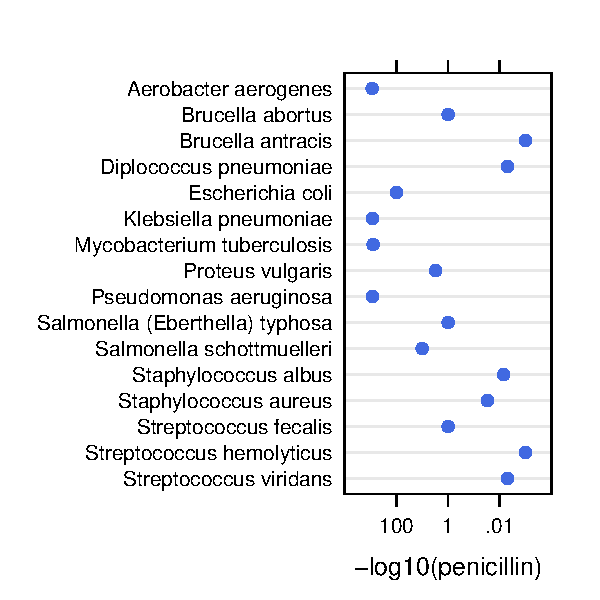
\includegraphics[width=\maxwidth]{figure/unnamed-chunk-5-1} 

}



\end{knitrout}


% ----------------------------------------------------------------------------

\section{Application to mixed models}

During the process of iterative fitting of mixed models, it is often useful
to compare fits of different models to data, for example using
loglikelihood or AIC values, or with the help of resiudal plots.
It can also be very informative to
inspect the variance components.  The \code{lucid} package provides a function
called \code{vc} that makes it easy to extract the estimated variances and
correlations from fitted models and prints them in friendly format
using the \code{lucid} function.

The \code{vc} function has methods that can be used with the
\code{nlme} \citep{pinheiro2014nlme},
\code{lme4} \citep{bates2014lme4}, and
\code{asreml} \citep{butler2009asreml}
packages.
The \code{VarCorr} function can be used to similar effect with the
\code{nlme} and \code{lme4} packages, but it shows variances for \code{nlme}
models and standard deviations for \code{lme4} models.
The \code{VarCorr} function is not available for the
\code{asreml} package.  The \code{vc} function provides a unified interface
for extracting the variance components from fitted models and prints
the results using \code{lucid}.

\cite{pearce1988manual} suggest showing four significant digits for the error
mean square and two decimal places digits for $F$ values.  The \code{lucid}
function uses a similar philosophy, presenting the
variances with four significant digits and \code{asreml} $Z$ statistics with
two significant digits.

The following simple example illustrates use of the \code{vc} function.

\begin{knitrout}
\definecolor{shadecolor}{rgb}{0.969, 0.969, 0.969}\color{fgcolor}\begin{kframe}
\begin{alltt}
\hlkwd{require}\hlstd{(}\hlstr{"nlme"}\hlstd{)}
\hlkwd{data}\hlstd{(Rail)}
\hlstd{mn} \hlkwb{<-} \hlkwd{lme}\hlstd{(travel}\hlopt{~}\hlnum{1}\hlstd{,} \hlkwc{random}\hlstd{=}\hlopt{~}\hlnum{1}\hlopt{|}\hlstd{Rail,} \hlkwc{data}\hlstd{=Rail)}
\hlkwd{vc}\hlstd{(mn)}
\end{alltt}
\begin{verbatim}
##       effect variance stddev
##  (Intercept)   615.3  24.81 
##     Residual    16.17  4.021
\end{verbatim}
\begin{alltt}
\hlkwd{require}\hlstd{(}\hlstr{"lme4"}\hlstd{)}
\hlstd{m4} \hlkwb{<-} \hlkwd{lmer}\hlstd{(travel}\hlopt{~}\hlnum{1} \hlopt{+} \hlstd{(}\hlnum{1}\hlopt{|}\hlstd{Rail),} \hlkwc{data}\hlstd{=Rail)}
\hlkwd{vc}\hlstd{(m4)}
\end{alltt}
\begin{verbatim}
##       grp        var1 var2   vcov  sdcor
##      Rail (Intercept) <NA> 615.3  24.81 
##  Residual        <NA> <NA>  16.17  4.021
\end{verbatim}
\begin{alltt}
\hlcom{#require("asreml")}
\hlcom{#ma <- asreml(travel~1, random=~Rail, data=Rail)}
\hlcom{#vc(ma)}
\hlcom{##         effect component std.error z.ratio constr}
\hlcom{##  Rail!Rail.var    615.3      392.6     1.6    pos}
\hlcom{##     R!variance     16.17       6.6     2.4    pos}
\end{alltt}
\end{kframe}
\end{knitrout}

A second example is more complex.  The example
is no longer reproducible due to changes in the mixed-models
software, so only the output is shown.  A single model was fit to
data using two different optimization methods.  The goal was to
compare the results from the two optimizers.  In the output below,
the first two columns identify terms in the model, the next two
columns are the variance and standard deviation from one optimizer,
while the final two columns are from the other optimizer.

The default printing is shown first.
\begin{knitrout}
\definecolor{shadecolor}{rgb}{0.969, 0.969, 0.969}\color{fgcolor}\begin{kframe}
\begin{alltt}
\hlkwd{cbind}\hlstd{(d1,d2[,}\hlnum{3}\hlopt{:}\hlnum{4}\hlstd{])}
\end{alltt}
\begin{verbatim}
##      Groups        Name  Variance Std.Dev. Variance   Std.Dev.
## 1   new.gen (Intercept)   2869.45   53.567 3.23e+03  56.818310
## 2       one       r1:c3   5531.60   74.375 7.69e+03  87.675211
## 3     one.1       r1:c2  58225.75  241.300 6.98e+04 264.123506
## 4     one.2       r1:c1 128003.60  357.776 1.07e+05 327.750047
## 5     one.3          c8   6455.77   80.348 6.79e+03  82.381314
## 6     one.4          c6   1399.73   37.413 1.64e+03  40.446339
## 7     one.5          c4   1791.65   42.328 1.23e+04 110.764195
## 8     one.6          c3   2548.89   50.486 2.69e+03  51.831045
## 9     one.7          c2   5941.80   77.083 7.64e+03  87.435345
## 10    one.8          c1      0.00    0.000 9.56e-04   0.030918
## 11    one.9         r10   1132.95   33.659 1.98e+03  44.446766
## 12   one.10          r8   1355.23   36.813 1.24e+03  35.234043
## 13   one.11          r4   2268.73   47.631 2.81e+03  53.020431
## 14   one.12          r2    241.79   15.550 9.28e+02  30.465617
## 15   one.13          r1   9199.94   95.916 1.04e+04 101.802960
## 16 Residual               4412.11   66.424 4.13e+03  64.240858
\end{verbatim}
\end{kframe}
\end{knitrout}
Do the two optimization methods give similar results?  It is difficult
to compare the results due to the clutter of extra digits, and even
more importantly, because of a quirk in the way R formats the output.
The variances in column 3 are shown in non-scientific format, while
the variances in column 5 are shown in scientific format!

The \code{lucid} function is now used to show the results.
\begin{knitrout}
\definecolor{shadecolor}{rgb}{0.969, 0.969, 0.969}\color{fgcolor}\begin{kframe}
\begin{alltt}
\hlkwd{lucid}\hlstd{(}\hlkwd{cbind}\hlstd{(d1,d2[,}\hlnum{3}\hlopt{:}\hlnum{4}\hlstd{]))}
\end{alltt}
\begin{verbatim}
##      Groups        Name Variance Std.Dev. Variance Std.Dev.
## 1   new.gen (Intercept)     2870     53.6     3230  56.8   
## 2       one       r1:c3     5530     74.4     7690  87.7   
## 3     one.1       r1:c2    58200    241      69800 264     
## 4     one.2       r1:c1   128000    358     107000 328     
## 5     one.3          c8     6460     80.3     6790  82.4   
## 6     one.4          c6     1400     37.4     1640  40.4   
## 7     one.5          c4     1790     42.3    12300 111     
## 8     one.6          c3     2550     50.5     2690  51.8   
## 9     one.7          c2     5940     77.1     7640  87.4   
## 10    one.8          c1        0      0          0   0.0309
## 11    one.9         r10     1130     33.7     1980  44.4   
## 12   one.10          r8     1360     36.8     1240  35.2   
## 13   one.11          r4     2270     47.6     2810  53     
## 14   one.12          r2      242     15.6      928  30.5   
## 15   one.13          r1     9200     95.9    10400 102     
## 16 Residual                 4410     66.4     4130  64.2
\end{verbatim}
\end{kframe}
\end{knitrout}
The formatting of the variance columns is now consistent and simplified
with fewer digits shown.  It is easy to compare the columns and see
that the two optimizers are giving quite different answers.

% ----------------------------------------------------------------------------

\section{Appendix}

Session information:
\begin{itemize}\raggedright
  \item R version 3.1.2 (2014-10-31), \verb|x86_64-w64-mingw32|
  \item Base packages: base, datasets, graphics, grDevices, methods, stats,
    utils
  \item Other packages: knitr~1.8, lattice~0.20-29, lme4~1.1-7, lucid~1.1,
    Matrix~1.1-4, nlme~3.1-118, Rcpp~0.11.3
  \item Loaded via a namespace (and not attached): evaluate~0.5.5, formatR~1.0,
    grid~3.1.2, highr~0.4, MASS~7.3-35, minqa~1.2.4, nloptr~1.0.4,
    splines~3.1.2, stringr~0.6.2, tools~3.1.2
\end{itemize}


\bibliography{lucid}
\end{document}
